%\affil{Departamento de F\'{i}sica, Universidad de los Andes, Cra. 1 No. 18A-10, Edificio Ip, Bogot\'a, Colombia}
%\email{mc.remolina197@uniandes.edu.co}
%\email{je.forero@uniandes.edu.co}

\documentclass[11pt,a4paper]{article}
\usepackage{graphicx}
\usepackage{amssymb}
\usepackage[latin1]{inputenc}    %% european characters can be used (Windows, old Linux)
\usepackage[T1]{fontenc}   %% get hyphenation and accented letters right

% do not change these lines:
\pagestyle{empty}                %% no page numbers!
\usepackage[left=35mm, right=35mm, top=15mm, bottom=20mm, noheadfoot]{geometry}

\begin{document}
\thispagestyle{empty}

\title{\textbf{Influence of galaxy rotation and outflows \\
			   in the Lyman Alpha spectral line}}
		
\author{Maria Camila Remolina-Gutierrez$^1$, Jaime E. Forero-Romero$^1$\\
	    mc.remolina197@uniandes.edu.co, \hspace{0.8mm} je.forero@uniandes.edu.co\\ 
		$^1$ Departamento de F\'{i}sica, Universidad de los Andes \\
		Cra. 1 No. 18A-10, Edificio Ip, Bogot\'a, Colombia}
\date{} % <--- leave date empty
\maketitle\thispagestyle{empty} %% <-- you need this for the first page
\textit{\textbf{Keywords - Galaxies: high-redshift, Lyman Alpha Emission, Galaxy Rotation, Galaxy Outflows, Radiative Transfer.}}\\

Young galaxies in the Universe have a strong Ly-$\alpha$ emission caused by the ionized Hydrogen atoms in their interstellar medium. When the spectrum of a galaxy has an intense peak around the Ly-$\alpha$ natural frequency ($2.46\times 10^{15}$ Hz) it is called a Lyman Alpha Emitter (LAE). Typical LAEs are very distant ($z \gtrsim 2$). This makes that all the data astronomers can obtain from them is their spectra, and from there all the physical information of the galaxy must be derived. Trying to solve this task requires the creation of a simplified and solid model. In this monograph I propose to consider LAEs as a spherical distribution of Hydrogen atoms that undergoes a solid body rotation and a radial expansion, as seen in Fig. \ref{model}. 

\begin{figure}[h]
	%uncomment next line to include a graphic file
	\centerline{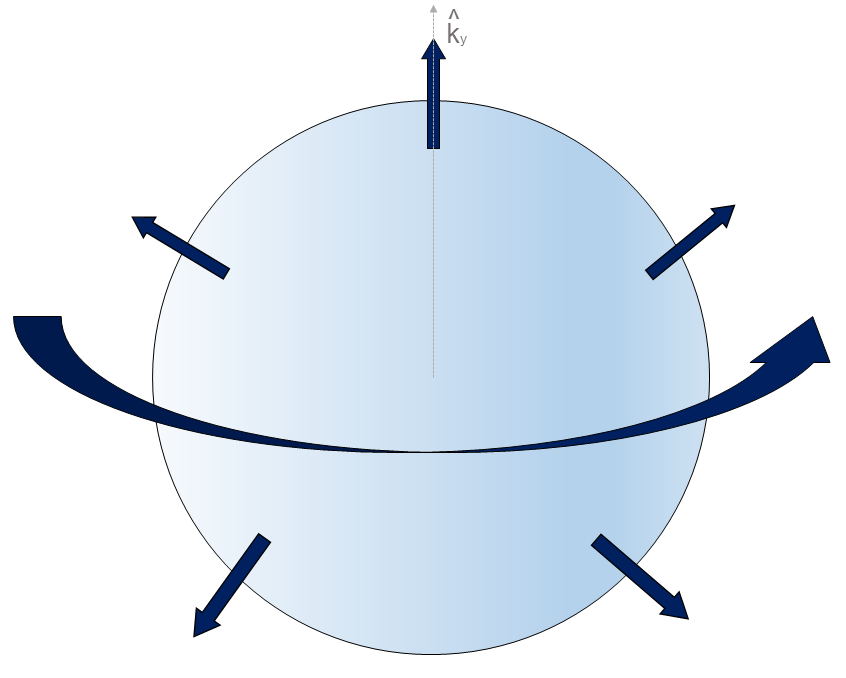
\includegraphics[width=4cm]{model.png}}
	\caption{Model of a Expanding and Rotating LAE.}
	\label{model}
\end{figure}

I simulate the effect of rotational velocity, outflow velocity and optical depth of the LAE in the outgoing spectra. The main conclusion is that this new model reproduces LAEs observed features in a clear way and with consistent physical parameters. However, proper observational fits are left for future work. This monograph accomplishes the objective of extracting as much information as possible from a LAE's Ly-$\alpha$ line.

%... a few optional references, such as \cite{Verhamme06}\\

%------------------------REFERENCES----------------------------

\bibliographystyle{latex/apj}
\bibliography{references}

\end{document}